\chapter{Results}
\label{ch_results}

These are the results I found from my investigation.

Present your results in a suitable format using tables and graphs where necessary. Remember to refer
to them in text and caption them properly.


\section{Simulation Results}


\section{Experimental Results}

\subsection{Focal Length of Lens}

The measured focal length of the lens was measured to be 53mm. Figure \ref{fig:focal_length_experiemnt_result} shows the focused point formed after adjusting the lens to 5.3cm above the working surface.

\begin{figure}[H]
	\centering
	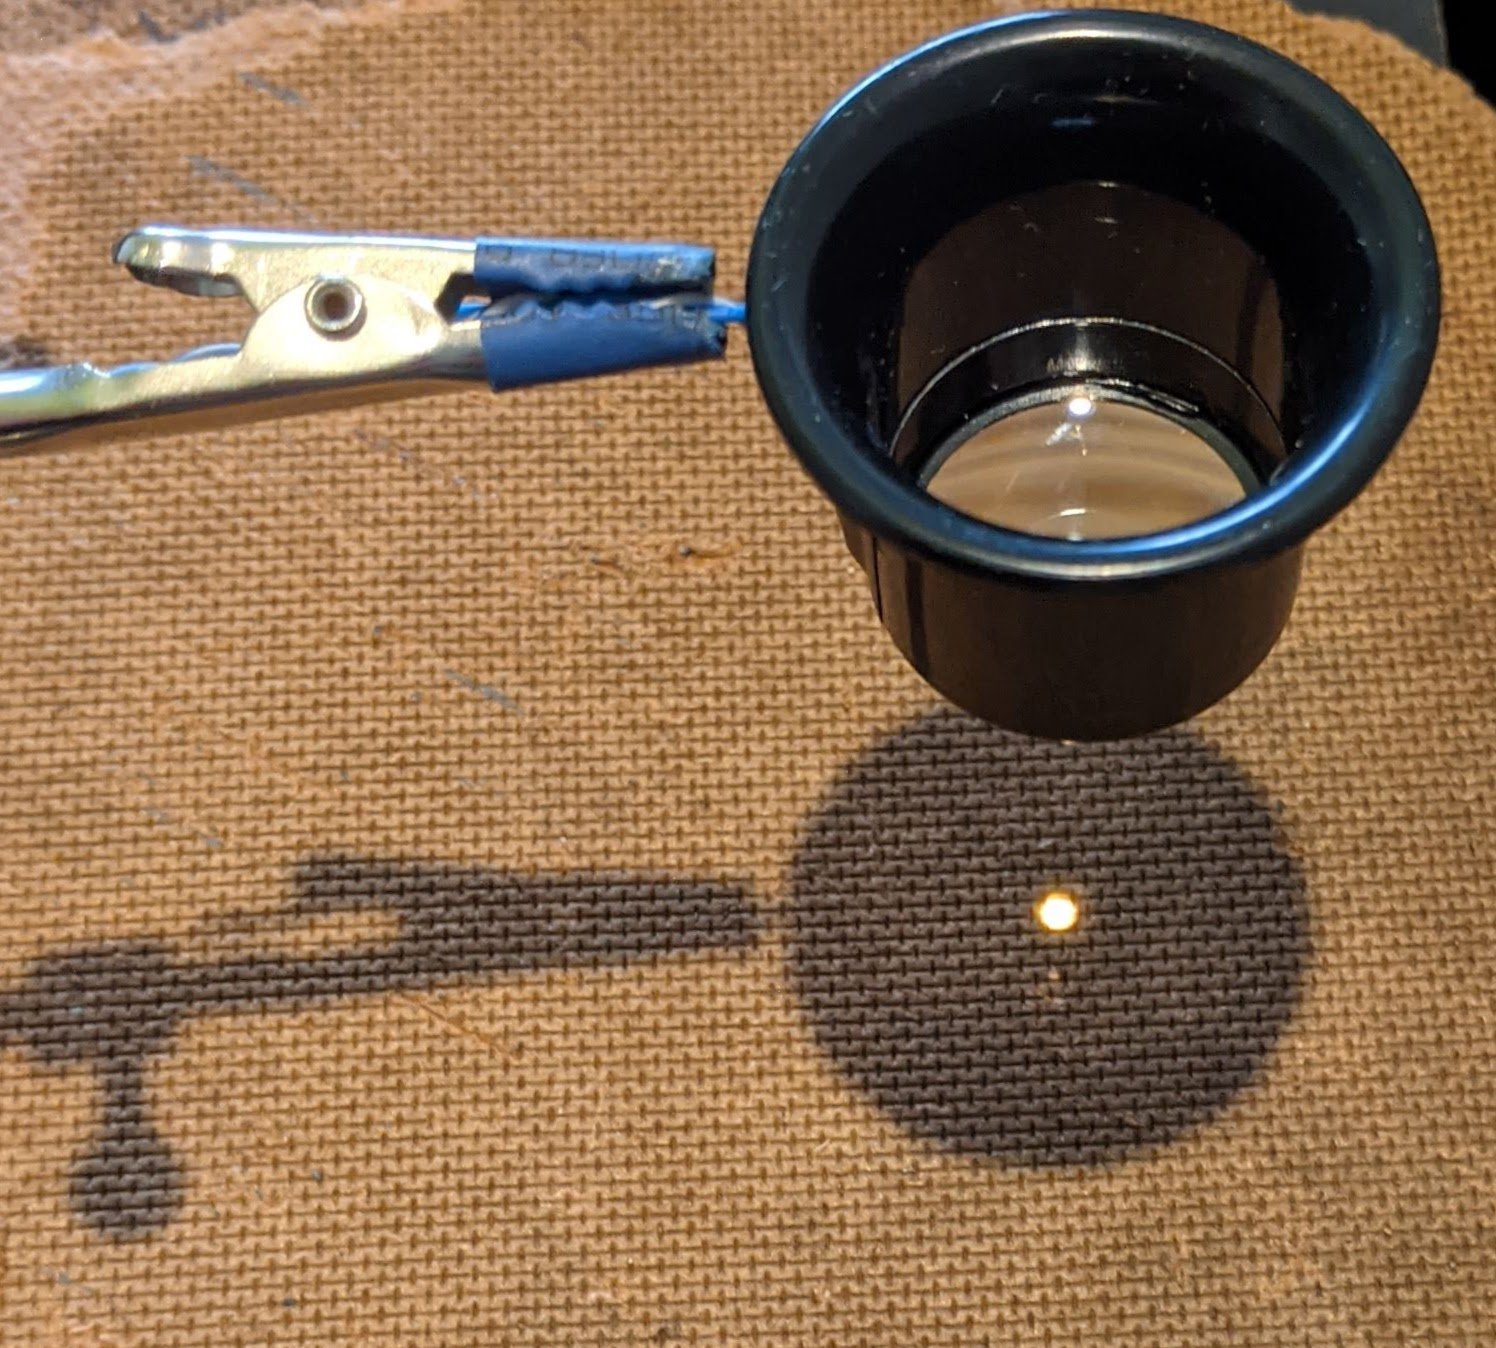
\includegraphics[width=.6\linewidth]{figures/results/focal_length_result.jpg}
	\captionof{figure}{Focal Length Experiemnt}
	\label{fig:focal_length_experiemnt_result}
\end{figure}


\subsection{Light Focus System}

Table \ref{label} below shows the beam spot size vs distance for the IR and warm-white power LEDs.

%table here

\subsection{Goertzel Filter Optimization}

\begin{figure}[H]
	\centering
	\begin{minipage}{.4\textwidth}
		%todo: make image higher quality after zoom
		\centering
		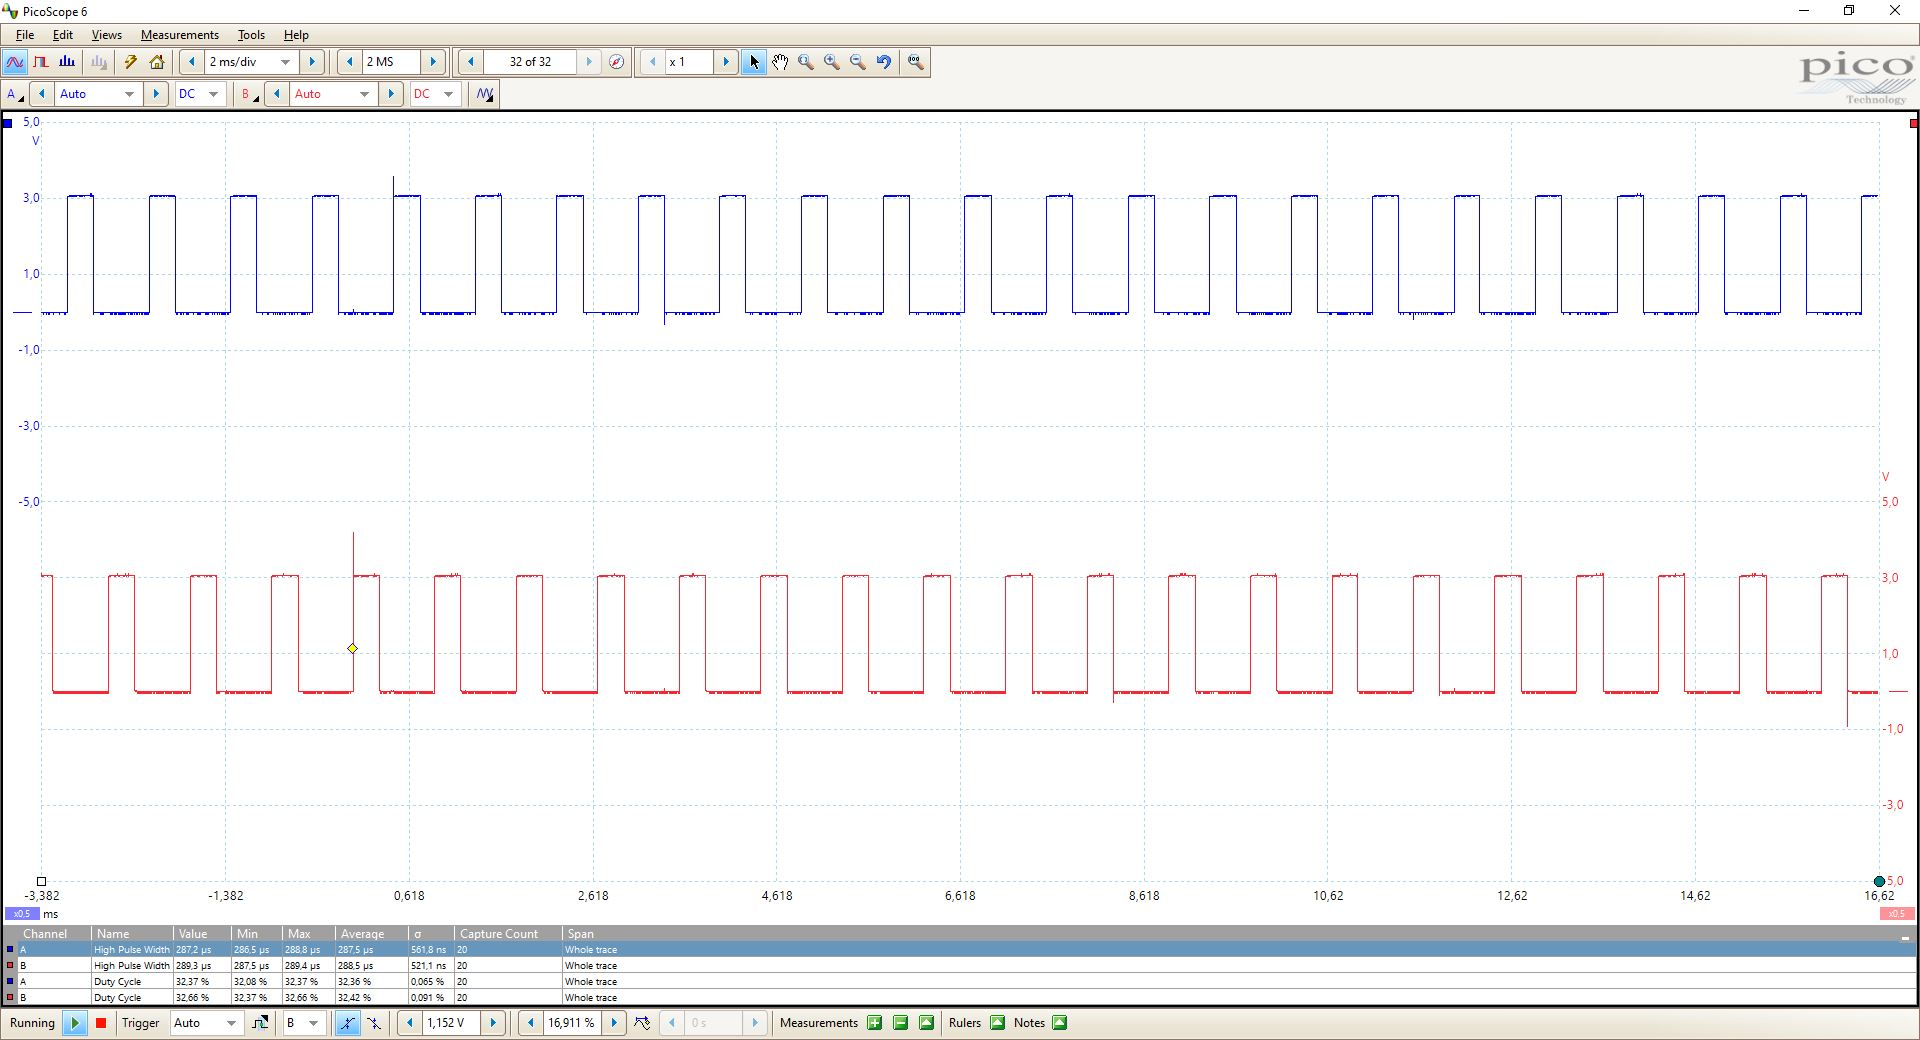
\includegraphics[width=0.9\linewidth]{figures/results/goertzel_filter_speed/16nu.JPG}
		\captionof{figure}{Scope Reading for unoptimized goertzel with $N = 16$}
		\label{fig:goertzel_speed_scope_screenshot}
	\end{minipage}%
	\hspace{.1\textwidth}
	\begin{minipage}{.4\textwidth}
		\begin{table}[H]
			\begin{tabular}{ccc}
				\hline
				\textbf{N} & \textbf{\begin{tabular}[c]{@{}c@{}}Unoptimized\\ ($\mu S$)\end{tabular}} & \textbf{\begin{tabular}[c]{@{}c@{}}Optimized\\ ($\mu S$)\end{tabular}} \\ \hline
				4 & 96.46 & 61.15 \\ \hline
				8 & 160.3 & 98.35 \\ \hline
				16 & 287.5 & 171.9 \\ \hline
				32 & 547.2 & 323.9 \\ \hline
				64 & 1059 & 621.1
			\end{tabular}
			\captionof{table}{Compiled results for goertzel speed experiemnt}
			\label{tbl:goertzel_speed_results}
		\end{table}
	\end{minipage}
\end{figure}

The results from the goertzel algorithm optimization experiment are tabulated in table \ref{tbl:goertzel_speed_results}, the adjacent screenshot shown in figure \ref{fig:goertzel_speed_scope_screenshot} illustrates the output recorded by the oscilloscope software during an iteration of the experiment. The recorded results are plotted in figure \ref{fig:goertzel_computation_plot} to provide graphical insight.

\begin{figure}[H]
	\centering
	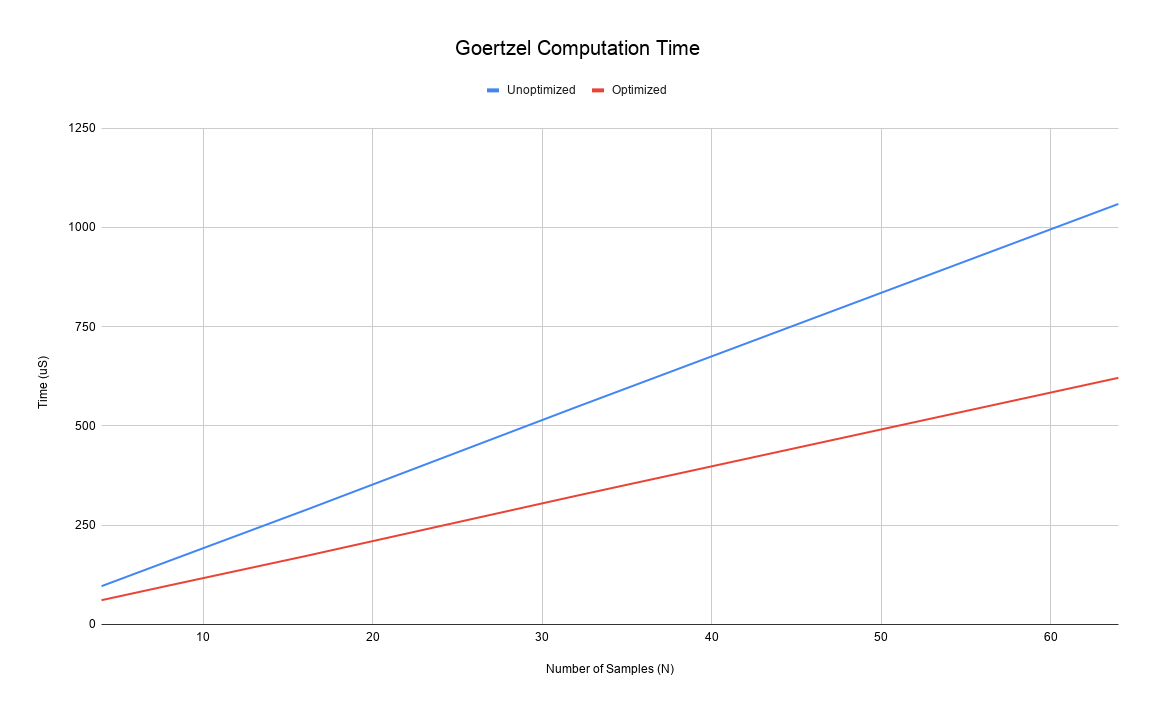
\includegraphics[width=\linewidth]{figures/results/goertzel_filter_speed/goertzel_computation_time.png}
	\captionof{figure}{Goertzel computation time versus sample set size}
	\label{fig:goertzel_computation_plot}
\end{figure}

Figure \ref{fig:goertzel_computation_plot} provides two important insights to the nature of the goertzel algorithm. The first observation may be found in the linearity of both plots, this confirms that both implementations of the algorithm have a time complexity of O(N) as noted in section \ref{sec:filter_optimization_design}. The practically perfect linearity in the results makes it possible to predict the timing requirements and make accurate theoretical predictions.

The gradient of the unoptimized curve is $16\mu S/sample$ and the gradient of the optimized curve is $9.3\mu S/sample$. The sampling rate used was $f_{sampling} \approx 144$kHz or $6.9\mu S/sample$. This indicates that even after optimizing the algorithm by simplifying out the multiplication step required for each new sample, the processor is still not fast enough to keep up with the rate of incoming samples.

The final observation is that the implemented optimization has two implications for the algorithms performance. The first implication is a small but non-zero constant timer saving, this comes as a result of removing the need for the multiplications to find the real and imaginary components of the k\textsubscript{th} DFT coefficient (see lines 18 and 19 of listing \ref{lst:goertzel_algorithm}). The second implication is a time difference which is directly proportional to the number of samples N, as indicated by the different gradients highlighted in the above paragraph.

\subsection{Goertzel Filter Performance}

An example, sampled sinusoid waveform is given in the appendix, figure \ref{fig:sampled_36khz_sinusoid}.

\begin{figure}[H]
	\centering
	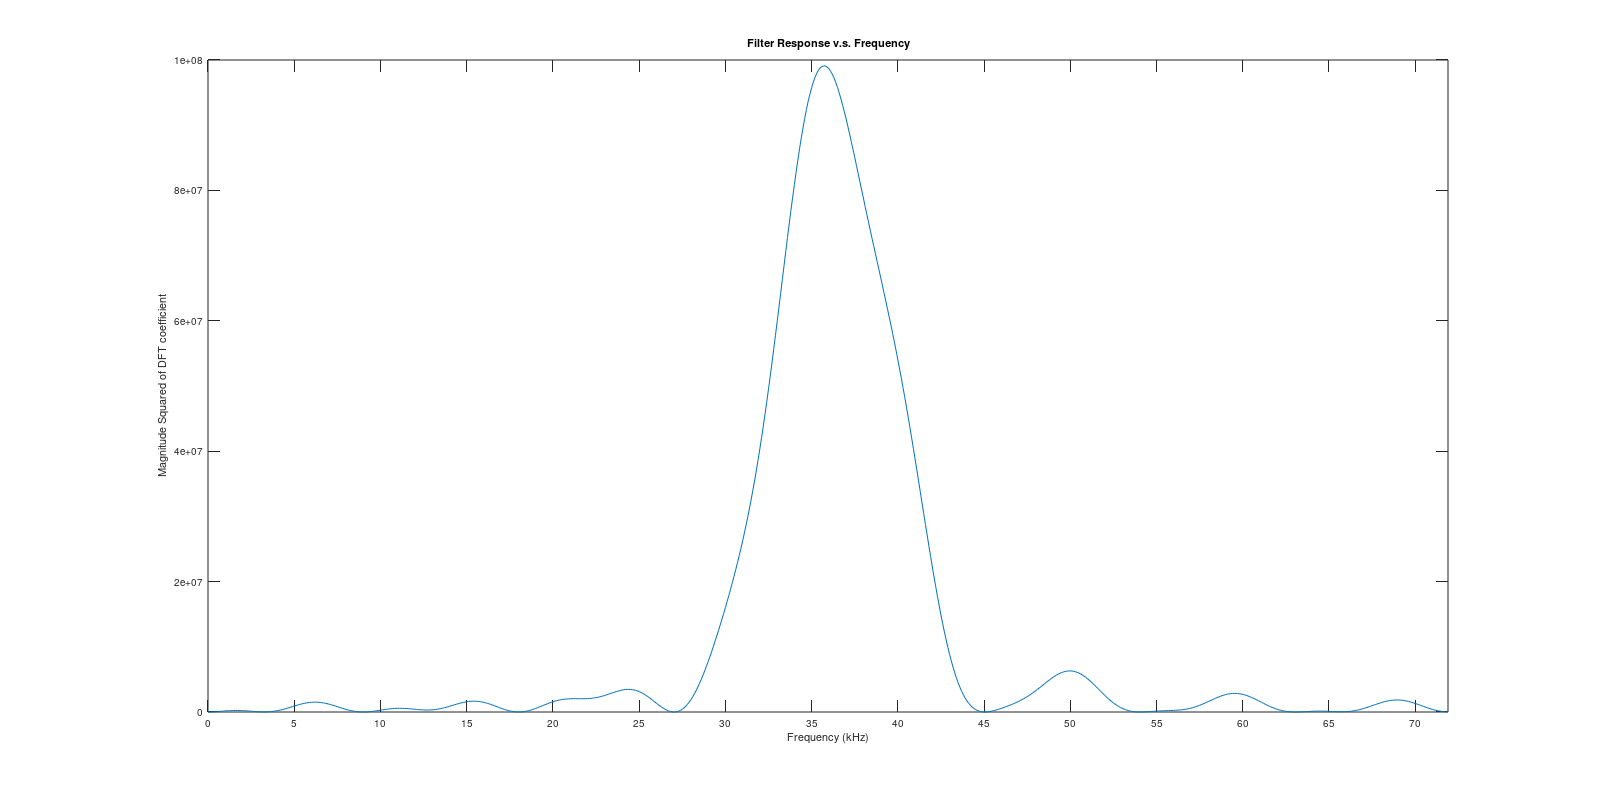
\includegraphics[width=\linewidth]{figures/results/goertzel_filter_simulation_wide.png}
	\caption{Frequency Response - Optimized Goertzel Algorithm}
	\label{fig:goertzel_filter_response}
\end{figure}



